%%%%%%%%%%%%%%%%%%%%%%%%%%%%%%%%%%%%%%%%%
% Two Column One Page Curriculum Vitae
% LaTeX Template
% Version 1.1 (24/1/13)
%
% This template has been downloaded from:
% http://www.LaTeXTemplates.com
%
% Original author:
% Alessandro (The CV Inn)
%
% IMPORTANT: THIS TEMPLATE NEEDS TO BE COMPILED WITH XeLaTeX
%
% This template uses several fonts not included with Windows/Linux by
% default. If you get compilation errors saying a font is missing, find the line
% on which the font is used and either change it to a font included with your
% operating system or comment the line out to use the default font.
% 
%%%%%%%%%%%%%%%%%%%%%%%%%%%%%%%%%%%%%%%%%

%----------------------------------------------------------------------------------------
%	PACKAGES AND OTHER DOCUMENT CONFIGURATIONS
%----------------------------------------------------------------------------------------

\documentclass[10pt]{article} % Font size - 10pt, 11pt or 12pt

\usepackage[hmargin=0.25cm, vmargin=1.25cm]{geometry} % Document margins

\usepackage{marvosym} % Required for symbols in the colored box
\usepackage{ifsym} % Required for symbols in the colored box
\usepackage{graphicx}
\graphicspath{ {images/} }
\usepackage[usenames,dvipsnames]{xcolor} % Allows the definition of hex colors

% Fonts and tweaks for XeLaTeX
\usepackage{fontspec,xltxtra,xunicode}
\defaultfontfeatures{Mapping=tex-text}
\setromanfont[Mapping=tex-text]{FreeSans} % Main document font
\setsansfont[Scale=MatchLowercase,Mapping=tex-text]{Purisa} % Font for your name at the top
%\setmonofont[Scale=MatchLowercase]{Andale Mono}

% Colors for links, text and headings
\usepackage{hyperref}
\definecolor{linkcolor}{HTML}{5881ee} % blue color for links
\definecolor{shade}{HTML}{F5DD9D} % Peach color for the contact information box
\definecolor{text1}{HTML}{2b2b2b} % Main document font color, off-black
\definecolor{headings}{HTML}{701112} % Dark red color for headings
% Other color palettes: shade=B9D7D9 and linkcolor=A40000; shade=D4D7FE and linkcolor=FF0080

\hypersetup{colorlinks,breaklinks, urlcolor=linkcolor, linkcolor=linkcolor} % Set up links and colors

\usepackage{fancyhdr}
\pagestyle{fancy}
\fancyhf{}
% Headers and footers can be added with the \lhead{} \rhead{} \lfoot{} \rfoot{} commands
% Example footer:
%\rfoot{\color{headings} {\sffamily Last update: \today}. Typeset with Xe\LaTeX}

%\renewcommand{\headrulewidth}{0pt} % Get rid of the default rule in the header

\usepackage{titlesec} % Allows creating custom \section's

% Format of the section titles
\titleformat{\section}{\color{headings}
\scshape\Large\raggedright}{}{0em}{}[\color{black}\titlerule]

\titlespacing{\section}{0pt}{0pt}{5pt} % Spacing around titles

\begin{document}

\color{text1} % Sets the default text color for the whole document to the color defined as 'text1'

%----------------------------------------------------------------------------------------
%	TITLE
%----------------------------------------------------------------------------------------

%\par{\centering{\sffamily\Huge Ariadni-Karolina Alexiou}\\ % Your name
%{\color{headings}\fontspec[Variant = 2]{FreeSans} Curriculum {Vit\fontspec[Variant = 3]{FreeSans}\ae}\\[15pt]\par} % Curriculum vitae text in the Zapfino font
	
%----------------------------------------------------------------------------------------

\begin{minipage}[t]{0.5\textwidth} % Start the left-hand side of the page
\vspace{0pt} % Trick for alignment
	
%----------------------------------------------------------------------------------------
%	EDUCATION
%----------------------------------------------------------------------------------------




%----------------------------------------------------------------------------------------
%	WORK EXPERIENCE
%----------------------------------------------------------------------------------------

\section{Work Experience} 

%------------------------------------------------
% WORK EXPERIENCE 1
%------------------------------------------------
{\raggedleft\textsc{March 2013 - June 2013}\par}

{\raggedright\large \textbf{Software Engineering Intern at Google, Z\"urich}\\
}

\normalsize{While looking around in the codebase I was honored to find that all my website urls were featured in it! Specifically as prime examples of content farms to train Google's spam detection algorithms.}\\
\\
{\raggedleft\textsc{September 2013 - June 2015}\par}

{\raggedright\large \textbf{Software Developer at Teralytics AG, Z\"urich}\\
}

\normalsize{Refactored the entire codebase for the better while coworker was on a roadtrip to Iran. Coworker still took all the credit. I took my laptop with me when I left.}
\\
\\
{\raggedleft\textsc{November 2015 - February 2017}\par}

{\raggedright\large \textbf{Lead Data Engineer at Tracktics GmbH, Z\"urich}\\
}

    \normalsize{Successful in assimilating company machines into botnets without anybody, not even myself, noticing, no matter which provider was used (AWS, IBM Bluemix).}
\\
\\

{\raggedleft\textsc{March 2017 - Present}\par}

{\raggedright\large \textbf{Software Engineer at siroop, Z\"urich}\\
}

\normalsize{Now, this company was great but it closed way too soon, one could say, in the flower of its youth. I am so sad about leaving, I will probably keep the laptop as well.}
\\
\\


\end{minipage} % End the left-hand side of the page
\hfill
\begin{minipage}[t]{0.44\textwidth} % Start the right-hand side of the page
\vspace{0pt} % Trick for alignment

%----------------------------------------------------------------------------------------
%	COLORED BOX
%----------------------------------------------------------------------------------------

\colorbox{shade}{\textcolor{text1}{
        \begin{tabular}{l|p{5.5cm}}
            \raisebox{-1.25cm}{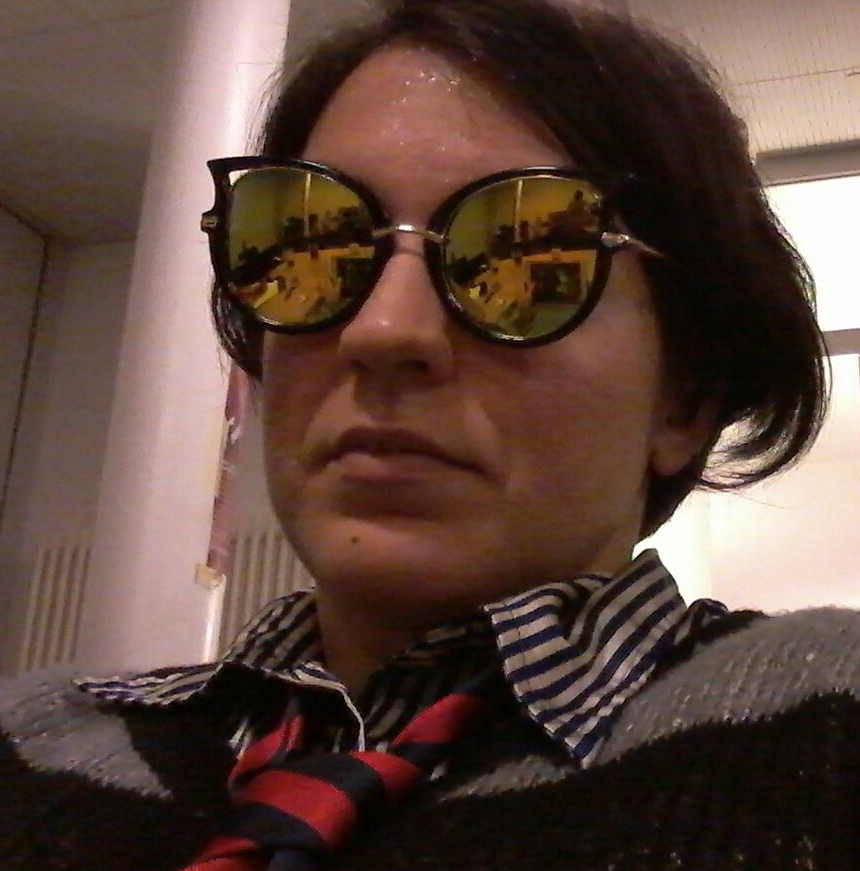
\includegraphics[height=2.5cm]{photo_2018}} &
        \begin{tabular}{l|p{5cm}}
    \raisebox{0pt}{\Smiley} & \textbf{Ariadni-Karolina Alexiou} \\ % Name
    \raisebox{-1pt}{\textifsymbol{18}} & Albisstrasse 35, Z\"urich 8038 \\ % Address
    \raisebox{-1pt}{\Mobilefone} & +41 76 227 1139\\ % Phone number
    \raisebox{-1pt}{\Letter} & carolinegr@gmail.com \\ % Email address
    \Keyboard & \href{http://www.github.com/carolinux}{http://www.github.com/carolinux} \\ % Github
        \end{tabular}  \\ % Name
\end{tabular}
}
}\\[10pt]





%----------------------------------------------------------------------------------------
%	COMPUTER SKILLS
%----------------------------------------------------------------------------------------


\section{Core Competencies} 
    \normalsize{\textbf{Content Farm Creation} - I was succesful in manually creating and profiting from content farms in the early 00s. Learning to program made it possible to create content farms with the best of them.}\\
\\
    \normalsize{\textbf{Not returning company hardware} (I get attached) }\\
\\
\normalsize{\textbf{Becoming part of a botnet} - I know exactly which security holes to leave open so that production machines can be up and mining cryptocurrencies for Russians in no time. }\\
\\
    \normalsize{\textbf{Attending remote meetings 2 minutes after waking up} (video off) }\\
\\
    \normalsize{\textbf{Team Player} - I am very good at refactoring code to my liking when coworkers are away on vacations.}\\
\\







	
\end{minipage} % End right-hand side of the page

\end{document}  
